\chapter{RESULTS AND DISCUSSION}

This chapter presents the experimental results of the Smart Gym Assistant. The
KNN model was evaluated using a reproducible stratified validation split covering
six classes: bicep bad, bicep good, bicep idle, squat bad, squat good, and squat
idle. The experiments compared different values of $k$ and different numbers of
representative prototypes per label.

\section{KNN Parameter Evaluation}
Figure~\ref{fig:results-accuracy} compares validation accuracy for five values of
$k$. Increasing the prototype count generally improves classification because the
stored examples represent a wider range of motion patterns. The highest observed
accuracy is approximately \textbf{89.06\%} with 128 prototypes per label and $k=3$.
The 64-prototype configuration used by the current embedded model achieves about
\textbf{80.56\%} at $k=5$, providing a smaller memory footprint for the ESP32.

\begin{figure}[H]
\centering
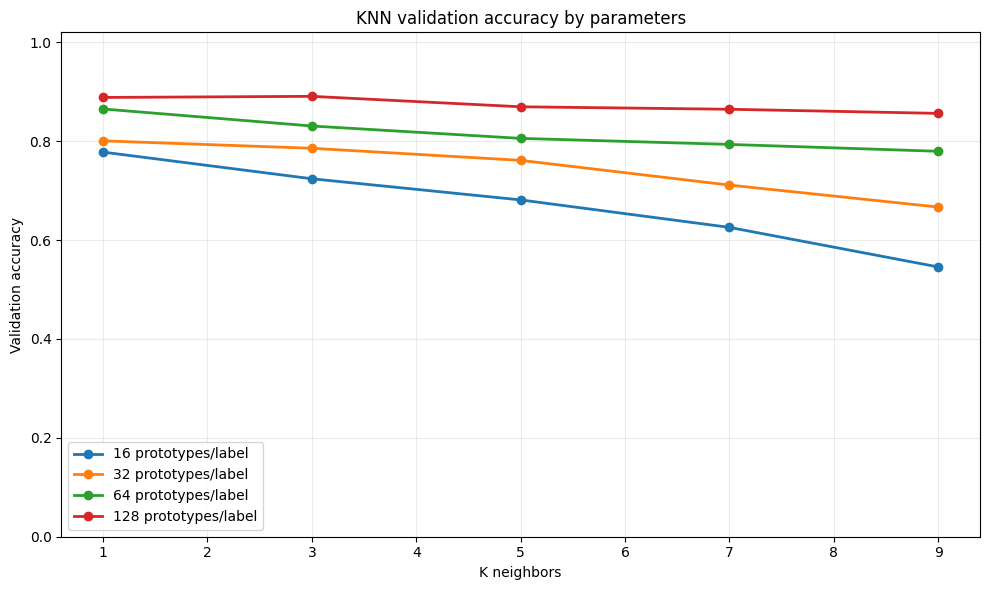
\includegraphics[width=0.88\textwidth]{Graphics/validation accuracy.png}
\caption{KNN validation accuracy for different parameter values.}
\label{fig:results-accuracy}
\end{figure}

The parameter-performance heatmap in Figure~\ref{fig:results-heatmap} gives the
same comparison in tabular visual form. It shows that larger prototype sets are
more accurate across the tested values of $k$, while excessively increasing $k$
reduces accuracy for this dataset. The final choice should therefore consider both
validation performance and the memory and computation available on the ESP32.

\begin{figure}[H]
\centering
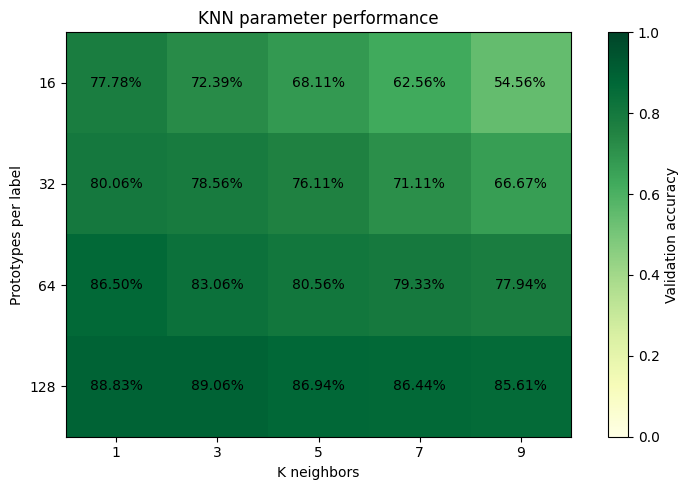
\includegraphics[width=0.78\textwidth]{Graphics/heatmap.png}
\caption{KNN parameter-performance heatmap.}
\label{fig:results-heatmap}
\end{figure}

\section{Class-Wise Performance}
The normalized confusion matrix in Figure~\ref{fig:results-confusion} and the
class-wise metrics give the following results:
\begin{itemize}
\item \textbf{Bicep bad:} 91.97\% precision, 84.00\% recall, and 87.80\% F1-score.
\item \textbf{Bicep good:} 84.66\% precision, 88.33\% recall, and 86.46\% F1-score.
\item \textbf{Bicep idle:} 91.51\% precision, 97.00\% recall, and 94.17\% F1-score.
\item \textbf{Squat bad:} 87.46\% precision, 81.33\% recall, and 84.28\% F1-score.
\item \textbf{Squat good:} 86.71\% precision, 87.00\% recall, and 86.86\% F1-score.
\item \textbf{Squat idle:} 92.06\% precision, 96.67\% recall, and 94.31\% F1-score.
\end{itemize}

The results can be interpreted as follows:
\begin{itemize}
\item The \textbf{idle classes} are recognized most consistently, with F1-scores above \textbf{94\%}.
\item Bicep idle has 97.0\% recall and squat idle has 96.7\% recall, showing that
	stationary samples are well separated from movement classes.
\item The main confusion occurs between bad and good posture within the same
	exercise. Squat bad is classified as squat good in approximately 12.3\% of
	samples, while squat good is classified as squat bad in approximately 10.0\%.
\item \textbf{Squat bad} has the lowest recall at \textbf{81.33\%} and the lowest F1-score at \textbf{84.28\%},
	so incorrect squat posture is the most difficult class to detect.
\item Bicep bad has high precision but lower recall, meaning that bad predictions
	are usually correct but some bad-posture samples are missed.
\item Additional bad-posture samples, clearer posture boundaries, and consistent
	sensor placement could improve safety-related feedback.
\end{itemize}

\begin{figure}[H]
\centering
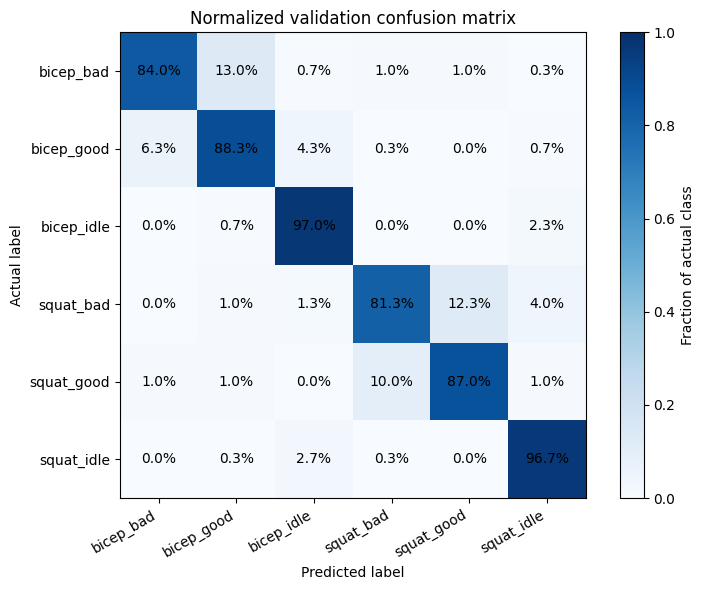
\includegraphics[width=0.78\textwidth]{Graphics/normalized validation confusin matrix.png}
\caption{Normalized validation confusion matrix.}
\label{fig:results-confusion}
\end{figure}

\section{Discussion}
The results demonstrate that a compact KNN classifier can distinguish exercise and
posture states from twelve inertial features. Batch voting improves the stability
of individual predictions, and local inference allows the ESP32 to provide OLED
and buzzer feedback without waiting for the network.

The results also show a practical trade-off. More prototypes improve validation
accuracy but require additional program memory and distance calculations. The
current 384-sample embedded model represents six labels with 64 samples each and
uses $k=5$, which is suitable for the available embedded resources. Additional
training data from different users, improved posture labeling, and a later model
export using the best validated parameters could improve generalization.
